\documentclass{article}
\usepackage{graphicx, mathtools, amsmath, amssymb, float, fancyhdr}
\usepackage{halloweenmath}
\graphicspath{{Images/}}

\setlength{\oddsidemargin}{0in}
\setlength{\textwidth}{6.5in}
\setlength{\topmargin}{-.55in}
\setlength{\textheight}{9in}
\pagestyle{fancy}

\makeatletter
\renewcommand*\env@matrix[1][*\c@MaxMatrixCols c]{%
  \hskip -\arraycolsep
  \let\@ifnextchar\new@ifnextchar
  \array{#1}}
\makeatother


\fancyfoot{}
\fancyhead[R]{$\mathbat$ \thepage \hspace{0.075cm} $\mathbat$}
\fancyhead[L]{$\mathbat$ MATH 5430 $\mathbat$}

\begin{document}
\begin{center}
    {\Huge Homework 3}
    \vspace{0.5cm}

    {\Large Michael Nameika}
\end{center}

\section*{Section 2.6 Problems}
\begin{itemize}
    \item[1.] Determine if the following functions satisfy a local or uniform Lipchitz condition.
    \begin{itemize}
        \item[(a)] $|y|$
        \newline\newline
        \textit{Soln.} $f(y) = |y|$ is globally Lipschitz. To see this, let $x,y \in \mathbb{R}$ and notice
        \[||x| - |y|| \leq |x - y|\]
        by the reverse triangle inequality. Thus, $|y|$ is globally Lipschitz with Lipschitz constant $L = 1$.
        
        \item[(b)] $\tan^{-1}(y)$
        \newline\newline
        \textit{Soln.} $f(y) = \tan^{-1}(y)$ is globally Lipschitz. To see this, let $x,y \in \mathbb{R}$. By the Mean Value Theorem, we have that there exists a $c \in (x,y)$ (or $(y,x)$) such that
        \[|\tan^{-1}(x) - \tan^{-1}(y)| = |f'(c)||x - y|.\]
        but 
        \[f'(c) = \frac{1}{1 + c^2}\]
        which is clearly bounded above by 1 for all $c \in \mathbb{R}$. That is,
        \[|\tan^{-1}(x) - \tan^{-1}(y)| \leq |x - y|\]
        so that $\tan^{-1}(y)$ is globally Lipschitz with Lipschitz constant $L = 1$. \hfill $\mathghost$
        

        \item[(c)] $\frac{t^2y}{1 + y^2}$
        \newline\newline
        \textit{Soln.} Notice that $f(t,y) = \frac{t^2y}{1 + y^2}$ is not globally Lipschitz in $t$ since for any fixed $y$, $f(t,y) = at^2$ with $a = \frac{y}{1 + y^2}$, $at^2$ is not a globally Lipchitz function. However, on a compact interval in $t$, $t^2$ is Lipschitz since $t^2$ is continuous. Now, $f(t,y)$ is globally Lipschitz in $y$. To see this, by the Mean Value Theorem, we have that 
        \[|f(t,b) - f(t,a)| = |f_y(t,c)||b - a|\]
        for some $c \in (a,b)$ (or $(b,a)$). We must find a bound for $f_y(t,c)$. To do so, we will find the critical points of $f_y(t,c)$. Notice
        \begin{align*}
            f_{yy}(t,y) &= \frac{2y(y^2 - 3)}{(1 + y^2)^3} = 0\\
            \implies 2y(y^2 - 3) &= 0
        \end{align*}
        thus, $y = 0, \pm \sqrt{3}$ are the critical points of $f_y$. Plugging these in, we find
        \[f_y(t,0) = t^2, \hspace{0.3em} f_y(t,\sqrt{3}) = \frac{\sqrt{3}}{16}t^2, \hspace{0.3em} f_y(t,-\sqrt{3}) = -\frac{\sqrt{3}}{16}t^2\]
        so that for any fixed $t$, $|f_y(t,y)| \leq t^2$. Hence, $f$ is globally Lipschitz. \hfill $\mathghost$
    \end{itemize}
    

    \item[2.] Find the maximal interval of existence for the differential equation
    \[y' = \frac{1}{1 + y^2}, \:\: y(0) = 0.\]
    Show that the exact solution supports your conclusion.
    \newline\newline
    \textit{Soln.} I claim that $f(y) = \frac{1}{1 + y^2}$ is globally Lipschitz. 
    \newline\newline
    \textit{Proof:} Let $a,b \in \mathbb{R}$. By the mean value theorem, we have that there exists some $c \in [a,b]$ (or $[b,a]$) such that
    \[|f(b) - f(a)| = |f'(c)||b - a|.\]
    We wish to find a bound for $f'(y)$ for all $y \in \mathbb{R}$. To do so, let us first find any critical points:
    \begin{align*}
        f''(y) &= \frac{1 - 3y^2}{(1 + y^2)^3} = 0
    \end{align*}
    which gives us $x = \pm \frac{1}{\sqrt{3}}$. Note that 
    \[f'\left(\frac{1}{\sqrt{3}}\right) = -f'\left(-\frac{1}{\sqrt{3}}\right) = -\frac{3\sqrt{3}}{8}\]
    and since 
    \[|f'(y)| \to 0 \text{  as  } y \to \infty\]
    we have that 
    \[|f'(y)| \leq \frac{3\sqrt{3}}{8}\]
    for all $y \in \mathbb{R}$. Thus,
    \[|f(b) - f(a)| \leq \frac{3\sqrt{3}}{8}|b - a|\]
    so that $f$ is globally Lipschitz with Lipschitz constant $L = \frac{3\sqrt{3}}{8}$. Hence, a unique global solution exists. \hfill $\mathghost$
    \newline\newline
    Inspecting the explicit solution, via separation of variables, we find
    \[y^3 + 3y - 3t = 0\]
    and by Cardano's formula, we have
    \[y = \sqrt[3]{\frac{3}{2}t + \sqrt{\frac{9}{4}t^2 + 1}} + \sqrt[3]{\frac{3}{2}t - \sqrt{\frac{9}{4}t^2 + 1}}\]
    which is clearly defined for all $t$. Below is a plot of the solution on $-10 \leq t \leq 10$:
    \begin{figure}[H]
        \centering
        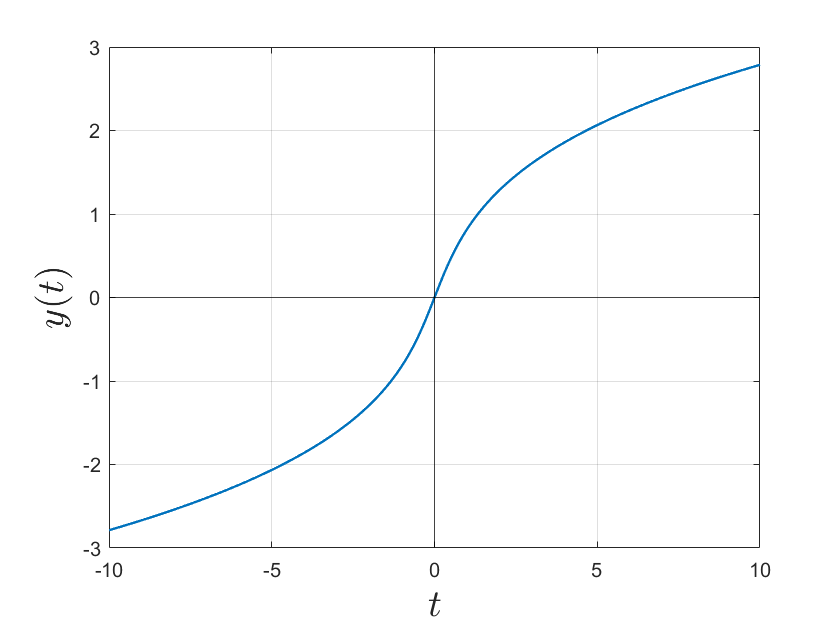
\includegraphics[scale = 0.3]{sampleSoln.png}
    \end{figure}
    
    
\end{itemize}

\section*{Section 2.7 Problems}
\begin{itemize}
    \item[3.] Compute the solution of the initial value problem $\dot{x} = t - x, x(0) = 1$, using the Euler and Runge-Kutta algorithms. Compare the results with the exact solution. Starting with $h = 0.1$, decrease $h$ and show that the methods are converging in an expected manner. 
    \newline\newline
    \textit{Soln.} Implementing Euler's method and RK4 into MATLAB to solve the system on the interval $[0,2]$, we find the following error plots for decreasing step sizes:
    \begin{figure}[H]
    \centering
        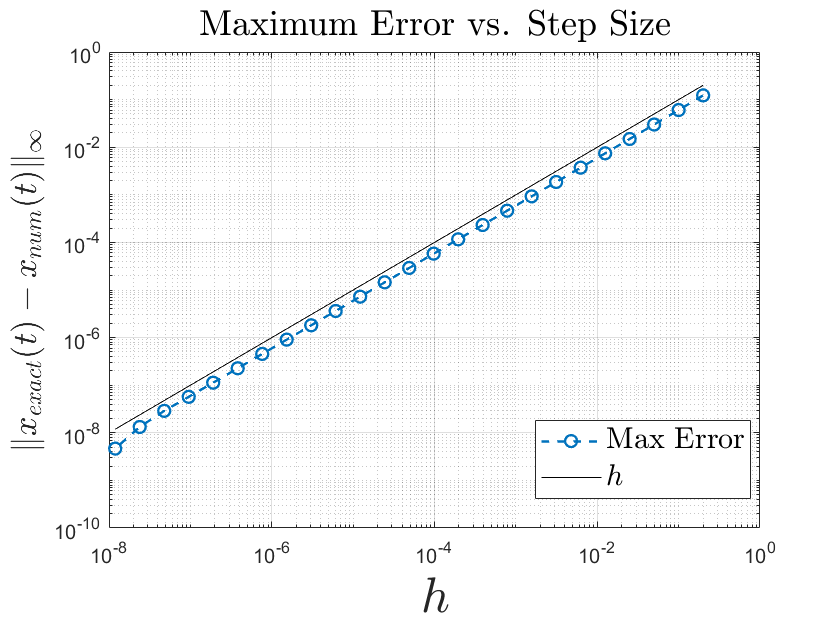
\includegraphics[scale = 0.3]{eulerError.png}
        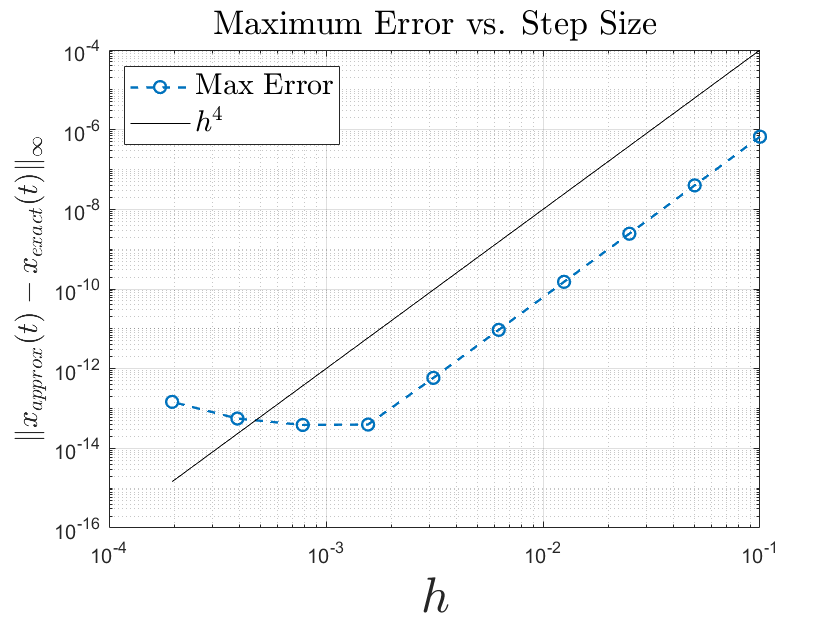
\includegraphics[scale = 0.3]{rk4Error.png}
        \newline
        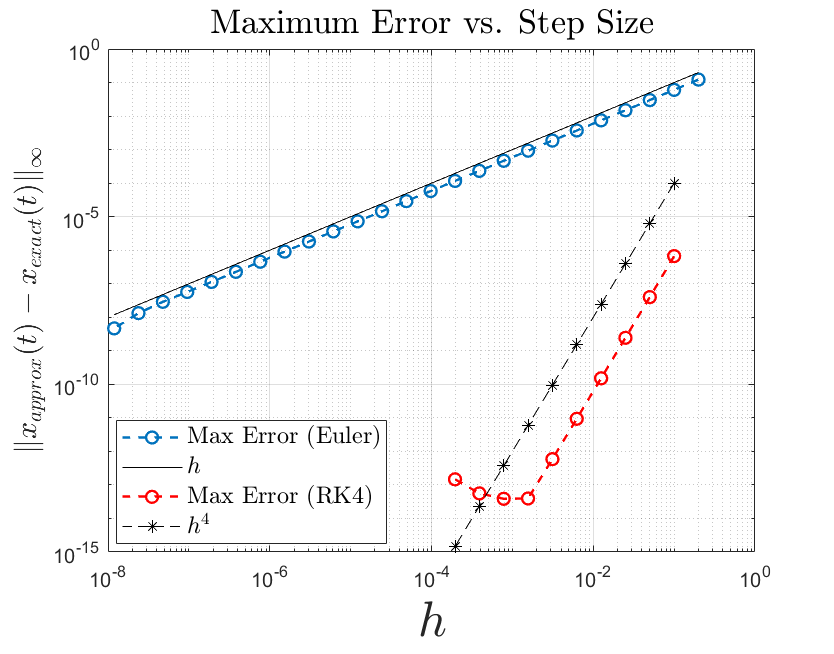
\includegraphics[scale = 0.3]{euler_rk4_error.png}
        \caption{Maximum errors versus step size for Euler and Rk4 methods, with them plotted together.}
    \end{figure}
    and the following plots of the numerical solution with the exact solution:
    \begin{figure}[H]
    \centering
        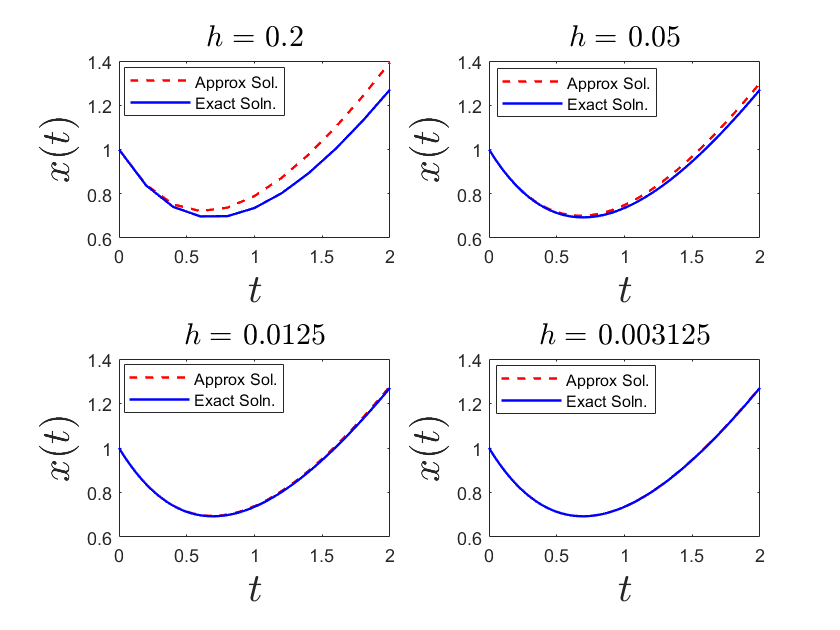
\includegraphics[scale = 0.5]{eulerConvergence.png}
        \newline
        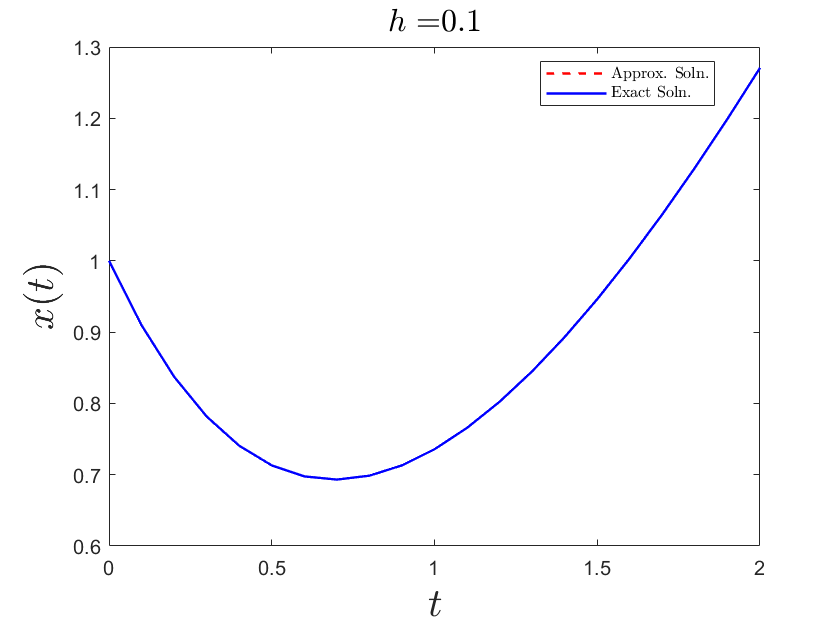
\includegraphics[scale = 0.3]{rk4Soln.png}
        \caption{Top: Convergence of the Euler method for decreasing step sizes. Bottom: Approximate and Exact solution with RK4.}
    \end{figure}
    \hfill $\mathghost$
\end{itemize}

\section*{Section 3.1 Problems}
\begin{itemize}
    \item[4.]\textbf{Grads only:} Show that the space of $n \times n$ matrices $\mathbb{C}^{n \times n}$ together with the matrix norm is a Banach space. Show (3.9).
    \newline\newline
    \textit{Proof:} To begin, we will show that the operator norm is indeed a norm. Let $X$ be a normed space and let $T : X \to X$ be a bounded linear operator on $X$. Define
    \[\|T\| = \sup_{\substack{x \in X \\ \|x\| = 1}} \|Tx\|.\]
    Note that $\|T\| \geq 0$ by definition of a norm on $X$. Now suppose $\|T\| = 0$. Then 
    \[\sup_{\substack{x \in X \\ \|x\| = 1}} \|Tx\| = 0\]
    so that
    \[0 \leq \|Tx\| \leq 0\]
    for all unit vectors $x \in X$. Thus, $T = 0$. Now let $\alpha$ be an arbitrary scalar and consider $\|\alpha T\|$. Notice
    \begin{align*}
        \|\alpha T\| &=\sup_{\substack{x \in X \\ \|x\| = 1}} \|\alpha (Tx)\| \tag*{(Def. scalar mult. of ops.)}\\
        &= \sup_{\substack{x \in X \\ \|x\| = 1}} |\alpha| \|Tx\| \tag*{(Homogeneity)}\\
        &= |\alpha| \sup_{\substack{x \in X \\ \|x\| = 1}} \|Tx\| \\
        &= |\alpha| \|T\|
    \end{align*}
    so homogeneity holds. Now, let $T,S : X \to X$ be bounded linear operators on $X$. Consider $\|T + S\|$:
    \begin{align*}
        \|T + S\| &= \sup_{\substack{x \in X \\ \|x\| = 1}} \|(T + S)(x)\| \tag*{(Def. add. of linear op.)}\\
        &= \sup_{\substack{x \in X \\ \|x\| = 1}} \|Tx + Sx\| \tag*{(Linearity)}\\
        &\leq \sup_{\substack{x \in X \\ \|x\| = 1}} (\|Tx\| + \|Sx\|)\\
        &\leq \sup_{\substack{x \in X \\ \|x\| = 1}} \|Tx\| + \sup_{\substack{x \in X \\ \|x\| = 1}}\|Sx\|\\
        &= \|T\| + \|S\|
    \end{align*}
    so that the triangle inequality holds. Thus, the operator norm is indeed a norm.
    \newline\newline
    Now we will show that the operator norm on an $n \times n$ matrix over $\mathbb{C}$ satisfies the following inequality:
    \[\max_{j,k} |A_{jk}| \leq \|A\| \leq n\max_{j,k}|A_{jk}|\]
    Let $x =(\alpha_1, \alpha_2, \cdots, \alpha_n)$ in $\mathbb{C}^n$ be such that $\|x\| = 1$. Then Notice
    \begin{align*}
        \|Ax\| &= \left\| \left(\sum_{k=1}^n A_{1k}\alpha_k, \sum_{k=1}^n A_{2k} \alpha_k, \cdots, \sum_{k=1}^n A_{nk}\alpha_k\right) \right\|\\
        &\leq \sum_{k=1}^n \left\|(A_{1k}\alpha_k, A_{2k}\alpha_k, \cdots, A_{nk}\alpha_k)\right\|\\
        &\leq \max_{j,k}|A_{jk}| \sum_{k=1}^n \|x\|\\
        &= n\max_{j,k} |A_{jk}|.
    \end{align*}
    And similarly, notice
    \begin{align*}
        \|Ax\| &= \left\| \left(\sum_{k=1}^n A_{1k}\alpha_k, \sum_{k=1}^n A_{2k} \alpha_k, \cdots, \sum_{k=1}^n A_{nk}\alpha_k\right) \right\|\\
        &\geq \max_{j,k}|A_{jk}|\|(\alpha_1, \alpha_2, \cdots, \alpha_n)\|\\
        &= \max_{j,k}|A_{jk}|\|x\|\\
        &= \max_{j,k}|A_{jk}|
    \end{align*}
    so we have
    \[\max_{j,k}|A_{j,k}| \leq \|Ax\| \leq n\max_{j,k}|A_{j,k}|\]
    hence, for $A$ to converge in $\mathbb{C}^{n\times n}$, it must be the case that each element of $A$ converges in $\mathbb{C}$. That is, if we have a Cauchy sequence of matrices $\{A_n\}$ in $\mathbb{C}^{n\times n}$, since $\mathbb{C}$ is complete, we have that each element-wise sequence of $\{A_n\}$ converges in $\mathbb{C}$, hence $A_n \to A \in \mathbb{C}^{n \times n}$. \hfill $\mathghost$
   
    
    
    
    \item[5.] Find a Jordan canonical form for the following matrix
    \[A = \begin{pmatrix*}[r]
        -3 & 1 & 0\\
        1 & -3 & -1\\
        0 & 1 & -3
    \end{pmatrix*}\]
    \textit{Soln.} Let us begin by finding the eigenvalues of $A$:
    \begin{align*}
        \det(A - \lambda I) &= \left|\begin{matrix}
            -3-\lambda & 1 & 0\\
            1 & -3-\lambda & -1\\
            0 & 1 & -3 - \lambda
        \end{matrix}\right|\\
        &= (-3 - \lambda)\left|\begin{matrix}
            -3-\lambda & -1\\
            1 & -3-\lambda
        \end{matrix}\right| - \left|\begin{matrix}
            1 & -1\\
            0 & -3 -\lambda
        \end{matrix}\right|\\
        &= (\lambda + 3)[-((\lambda + 3)^2 + 1) + 1]\\
        &= (\lambda+3)[-(\lambda + 3)^2 - 1 + 1]\\
        &= -(\lambda + 3)^3\\
        &= 0\\
        \implies \lambda_1,\lambda_2,\lambda_3 &= -3.
    \end{align*}
    So we have our Jordan matrix:
    \[J = \begin{pmatrix}
        -3 & 1 & 0\\
        0 & -3 & 1\\
        0 & 0 & -3
    \end{pmatrix}\]
    and we must now find the generalized eigenvectors to build the $U$ and $U^{-1}$ matrices. Let us begin by finding the true eigenvector associated with $\lambda_1 = -3$:
    \begin{align*}
        (A - \lambda_1)v_1 = 0
        \iff \begin{pmatrix}
            0 & 1 & 0\\
            1 & 0 & -1\\
            0 & 1 & 0
        \end{pmatrix}v_1 &= 0
    \end{align*}
    Denote $v_1 = (v_1^{(1)}, v_1^{(2)}, v_1^{(3)})^T$, it is clear from the above system that $v_1^{(2)} = 0$ and $v_1^{(1)} = v_1^{(3)}$. Set $v_1^{(3)} = 1$ so that
    \[v_1 = \begin{pmatrix}
        1\\
        0\\
        1
    \end{pmatrix}.\]
    We must now find the generalized eigenvectors, $w_2, w_3$. Finding $w_2$, we have
    \begin{align*}
        \begin{pmatrix}
            0 & 1 & 0\\
            1 & 0 & -1\\
            0 & 1 & 0
        \end{pmatrix}\begin{pmatrix}
            w_2^{(1)}\\
            w_2^{(2)}\\
            w_2^{(3)}
        \end{pmatrix} &= \begin{pmatrix}
            1\\
            0\\
            1
        \end{pmatrix}\\
        &\equiv \begin{pmatrix}[ccc|c]
            0 & 1 & 0 & 1\\
            1 & 0 & -1 & 0\\
            0 & 1 & 0 & 1
        \end{pmatrix}
    \end{align*}
    which gives us $w_2^{(2)} = 1$ and $w_2^{(1)} = w_2^{(3)}$. Set $w_2^{(3)} = 1$ so that
    \begin{align*}
        w_2 &= \begin{pmatrix}
            1\\
            1\\
            1
        \end{pmatrix}\\
        &= \begin{pmatrix}
            0\\
            1\\
            0
        \end{pmatrix} + v_1
    \end{align*}
    so take $w_2 = (0,1,0)^T$. We must now find the final generalized eigenvector, $w_3$:
    \begin{align*}
        \begin{pmatrix}
            0 & 1 & 0\\
            1 & 0 & -1\\
            0 & 1 & 0
        \end{pmatrix}\begin{pmatrix}
            w_3^{(1)}\\
            w_3^{(2)}\\
            w_3^{(3)}
        \end{pmatrix} &= \begin{pmatrix}
            0 \\
            1\\
            0
        \end{pmatrix}\\
        &\equiv \begin{pmatrix}[ccc|c]
            0 & 1 & 0 & 0\\
            1 & 0 & -1 & 1\\
            0 & 1 & 0 & 0
        \end{pmatrix}
    \end{align*}
    which gives us $w_3^{(2)} = 0$ and $w_3^{(1)} = 1 + w_3^{(3)}$. Set $w_3^{(3)} = 1$ so that $w_3^{(1)} = 2$ and so
    \begin{align*}
        w_3 &= \begin{pmatrix}
            2\\
            0\\
            1
        \end{pmatrix}.
    \end{align*}
    Setting $U = [v_1 \hspace{0.2em} | \hspace{0.2em} w_2 \hspace{0.2em} | \hspace{0.2em} w_3]$, 
    \[U = \begin{pmatrix}
        1 & 0 & 2\\
        0 & 1 & 0\\
        1 & 0 & 1
    \end{pmatrix}\]
    Inverting, we find
    \[U^{-1} = \begin{pmatrix}
        -1 & 0 & 2\\
        0 & 1 & 0\\
        1 & 0 & -1
    \end{pmatrix}\]
    so that, finally, we have
    \[A = \begin{pmatrix}
        1 & 0 & 2\\
        0 & 1 & 0\\
        1 & 0 & 1
    \end{pmatrix}\begin{pmatrix}
        -3 & 1 & 0\\
        0 & -3 & 1\\
        0 & 0 & -3
    \end{pmatrix}\begin{pmatrix}
        -1 & 0 & 2\\
        0 & 1 & 0\\
        1 & 0 & -1
    \end{pmatrix}\]
    \hfill $\mathghost$
    
    \item[6.] Write down all $3 \times 3$ Jordan matrices that have eigenvalues 2 and 5 (and no others).
    \newline\newline
    \textit{Soln.} We can have either 5 or 2 as a repeated eigenvalue, so the only $3\times 3$ Jordan matrices that have 2 and 5 as eigenvalues are
    \[\begin{pmatrix}
        2 & 0 & 0\\
        0 & 5 & 1\\
        0 & 0 & 5
    \end{pmatrix}, \hspace{1em}
    \begin{pmatrix}
        2 & 1 & 0\\
        0 & 2 & 0\\
        0 & 0 & 5
    \end{pmatrix}, \hspace{1em}
    \begin{pmatrix}
        5 & 1 & 0\\
        0 & 5 & 0\\
        0 & 0 & 2
    \end{pmatrix}, \hspace{1em}
    \begin{pmatrix}
        5 & 0 & 0\\
        0 & 2 & 1\\
        0 & 0 & 2
    \end{pmatrix}\]
    If the repeated eigenvalues have distinct eigenvectors, that is, the geometric multiplicity is equal to the algebraic multiplicity, we have
    \[\begin{pmatrix}
        5 & 0 & 0\\
        0 & 5 & 0\\
        0 & 0 & 2
    \end{pmatrix} \hspace{1em}
    \begin{pmatrix}
        2 & 0 & 0\\
        0 & 5 & 0\\
        0 & 0 & 5
    \end{pmatrix}\hspace{1em}
    \begin{pmatrix}
        2 & 0 & 0\\
        0 & 2 & 0\\
        0 & 0 & 5
    \end{pmatrix}\hspace{1em}
    \begin{pmatrix}
        5 & 0 & 0\\
        0 & 5 & 0\\
        0 & 0 & 2
    \end{pmatrix}\]
    \hfill $\mathghost$
    
    \item[7.] Compute the matrix exponential $\exp(A)$ for the matrix in question 5.
    \newline\newline
    \textit{Soln.} Recall that $\exp(UJU^{-1}) = U\exp(J)U^{-1}$ so that $\exp(A)$ from question 5 has the form
    \begin{align*}
        \exp(A) &= \begin{pmatrix}
            1 & 0 & 2\\
            0 & 1 & 0\\
            1 & 0 & 1
        \end{pmatrix}\exp\begin{pmatrix}
            -3 & 1 & 0\\
            0 & -3 & 1\\
            0 & 0 & -3
        \end{pmatrix}\begin{pmatrix}
            -1 & 0 & 2\\
            0 & 1 & 0\\
            1 & 0 & -1
        \end{pmatrix}.
    \end{align*}
    So all we need to find is $\exp(J)$. Notice we may rewrite
    \[J = -3I + N\]
    where 
    \[N = \begin{pmatrix}
        0 & 1 & 0\\
        0 & 0 & 1\\
        0 & 0 & 0
    \end{pmatrix}\]
    and that since $I$ commutes with any other matrix, $\exp(J) = \exp(-3I + N) = \exp(-3I)\exp(N)$. Notice that 
    \[N^2 = \begin{pmatrix}
        0 & 0 & 1\\
        0 & 0 & 0\\
        0 & 0 & 0
    \end{pmatrix}, \hspace{1em} N^3 = \begin{pmatrix}
        0 & 0 & 0\\
        0 & 0 & 0\\
        0 & 0 & 0
    \end{pmatrix}\]
    so that 
    \[\exp(N) = \begin{pmatrix}
        1 & 1 & \frac{1}{2}\\
        0 & 1 & 1\\
        0 & 0 & 1
    \end{pmatrix}.\] Thus,
    \[\exp(J) = \begin{pmatrix}
        e^{-3} & e^{-3} & \frac{1}{2}e^{-3}\\
        0 & e^{-3} & e^{-3}\\
        0 & 0 & e^{-3}
    \end{pmatrix}\]
    and so
    \begin{align*}
        \exp(A) &= \begin{pmatrix}
            1 & 0 & 2\\
            0 & 1 & 0\\
            1 & 0 & 1
        \end{pmatrix}
        \begin{pmatrix}
            e^{-3} & e^{-3} & \frac{1}{2}e^{-3}\\
            0 & e^{-3} & e^{-3}\\
            0 & 0 & e^{-3}
        \end{pmatrix}\begin{pmatrix}
            -1 & 0 & 2\\
            0 & 1 & 0\\
            1 & 0 & -1
        \end{pmatrix}\\
        &= \begin{pmatrix}
            1 & 0 & 2\\
            0 & 1 & 0\\
            1 & 0 & 1
        \end{pmatrix}\begin{pmatrix}
            -\frac{1}{2}e^{-3} & e^{-3} & \frac{3}{2}e^{-3}\\
            e^{-3} & e^{-3} & -e^{-3}\\
            e^{-3} & 0 & -e^{-3}
        \end{pmatrix}\\
        &= \begin{pmatrix}
            \frac{3}{2}e^{-3} & e^{-3} & -\frac{1}{2}e^{-3}\\
            e^{-3} & e^{-3} & -e^{-3}\\
            \frac{1}{2}e^{-3} & e^{-3} & \frac{1}{2}e^{-3}
        \end{pmatrix}
    \end{align*}
    \hfill $\mathghost$
\end{itemize}


\section*{Section 3.2 Problems}
\begin{itemize}
    \item[8.] Solve the initial value problem $\dot{\mathbf{x}} = A\mathbf{x}(t),$ $\mathbf{x}(0) = \mathbf{x}_0$ for the following matrices. Be as explicit as possible in your representation of the solution. What is the solution behavior as $t \to \infty$?
    \begin{itemize}
        \item[(a)] $A = \begin{pmatrix}
            1 & -2\\
            -2 & 1
        \end{pmatrix}$
        \newline\newline
        \textit{Soln.} We begin by finding the eigenvalues of $A$:
        \begin{align*}
            \left|\begin{matrix}
                1 - \lambda & -2\\
                -2 & 1 - \lambda
            \end{matrix}\right| &= (1 - \lambda)^2 - 4 = 0\\
            \implies (\lambda - 1)^2 &= 4\\
            \lambda - 1 &= \pm 2\\
            \lambda = 1 \pm 2
        \end{align*}
        so $\lambda_1 = 3$, $\lambda_2 = -1$ which are real, distinct eigenvalues. Finding the associated eigenvectors, we have, for $\lambda_1$,
        \begin{align*}
            (A - \lambda_1I)u_1 &= \begin{pmatrix}
                -2 & -2\\
                -2 & -2
            \end{pmatrix}\begin{pmatrix}
                u_1^{(1)}\\
                u_1^{(2)}
            \end{pmatrix} = 0
        \end{align*}
        solving the above system, we have $u_1^{(1)} = -u_1^{(2)}$, and letting $u_1^{(2)} = 1$, we have
        \[u_1 = \begin{pmatrix}
            -1\\
            1
        \end{pmatrix}.\]
        Now, for $\lambda_2$, we have
        \[(A - \lambda_2I)u_2 = \begin{pmatrix}
            2 & -2\\
            -2 & 2
        \end{pmatrix}\begin{pmatrix}
            u_2^{(1)}\\
            u_2^{(2)}
        \end{pmatrix} = 0\]
        Solving, we have $u_2^{(1)} = u_2^{(2)}$, and letting $u_2^{(2)} = 1$, we find
        \[u_2^{(2)} = \begin{pmatrix}
            1\\
            1
        \end{pmatrix}.\]
        Then
        \[U = \begin{pmatrix}
            -1 & 1\\
            1 & 1
        \end{pmatrix}\]
        and so
        \[U^{-1} = \frac{1}{2}\begin{pmatrix}
            -1 & 1\\
            1 & 1
        \end{pmatrix}.\]
        Thus,
        \[A = \frac{1}{2}\begin{pmatrix}
            -1 & 1\\
            1 & 1
        \end{pmatrix}\begin{pmatrix}
            3 & 0\\
            0 & -1
        \end{pmatrix}\begin{pmatrix}
            -1 & 1\\
            1 & 1
        \end{pmatrix}.\]
        And since the solution to our system has the form
        \[\mathbf{x}(t) = \exp(tA)\mathbf{x}_0 = U\exp(tJ)U^{-1}\mathbf{x}_0\]
        we have
        \begin{align*}
            x(t) &= \frac{1}{2}\begin{pmatrix}
                -1 & 1\\
                1 & 1
            \end{pmatrix}\begin{pmatrix}
                3 & 0\\
                0 & -1
            \end{pmatrix}\begin{pmatrix}
                -1 & 1\\
                1 & 1
            \end{pmatrix}\begin{pmatrix}
                x_{0,1}\\
                x_{0,2}
            \end{pmatrix}\\
            &= \frac{1}{2}\begin{pmatrix}
                -1 & 1\\
                1 & 1
            \end{pmatrix}\begin{pmatrix}
                -e^{3t} & e^{3t}\\
                e^{-t} & e^{-t}
            \end{pmatrix}\begin{pmatrix}
                x_{0,1}\\
                x_{0,2}
            \end{pmatrix}\\
            &= \frac{1}{2}\begin{pmatrix}
                -e^{3t} + e^{-t} & e^{-t} - e^{3t}\\
                e^{-t} - e^{3t} & e^{3t} + e^{-t}
            \end{pmatrix}\begin{pmatrix}
                x_{0,1}\\
                x_{0,2}
            \end{pmatrix}.
        \end{align*}
        Notice, if $x_0 = u_1$, the above system becomes
        \begin{align*}
            x(t) &= \frac{1}{2}\begin{pmatrix}
                e^{3t} + e^{-t} & e^{-t} - e^{3t}\\
                e^{-t} - e^{3t} & e^{3t} + e^{-t}
            \end{pmatrix}\begin{pmatrix}
                -1\\
                1
            \end{pmatrix}\\
            &= \frac{1}{2}\begin{pmatrix}
                -2e^{3t}\\
                2e^{3t}
            \end{pmatrix}\\
            &= e^{3t}u_1
        \end{align*}
        so that, as $t \to \infty$, $x_1(t) \to -\infty$ and $x_2(t) \to +\infty$. Similarly, if $x_0 = u_2$, we have
        \begin{align*}
            x(t) &= \frac{1}{2}\begin{pmatrix}
                e^{3t} + e^{-t} & e^{-t} - e^{3t}\\
                e^{-t} - e^{3t} & e^{3t} + e^{-t}
            \end{pmatrix}\begin{pmatrix}
                1\\
                1
            \end{pmatrix}\\
            &= \frac{1}{2}\begin{pmatrix}
                2e^{-t}\\
                2e^{-t}
            \end{pmatrix}\\
            &= e^{-t}u_2
        \end{align*}
        so that, as $t \to \infty$, $x(t) \to 0$. Note that if an initial condition is a linear combination of $u_1$ and $u_2$, the solution behavior from the $u_1$ component will dominate as $t \to \infty$ and the solution will tend to $\pm \infty$. \hfill $\mathghost$


        \item[(b)] $A = \begin{pmatrix}
            3 & -2\\
            1 & 1
        \end{pmatrix}$
        \newline\newline
        Let us begin by computing the eigenvalues for $A$:
        \begin{align*}
            \left|\begin{matrix}
                3 - \lambda & -2\\
                1 & 1 - \lambda
            \end{matrix}\right| &= (3 - \lambda)(1 - \lambda) + 2 = 0\\
            \implies \lambda^2 - 4\lambda + 5 &= 0\\
            \lambda^2 - 4\lambda + 4 &= -1\\
            (\lambda - 2)^2 &= -1\\
            \lambda = 2 \pm i
        \end{align*}
        so we have a complete set of complex eigenvalues. Now let us find the eigenvector corresponding to the eigenvalue $\lambda_1 = 2 + i$:
        \begin{align*}
            &\begin{pmatrix}
                1 - i & -2\\
                1 & -1 - i
            \end{pmatrix}\begin{matrix}
                R_1 - R_2 \to R_1\\
            \end{matrix}\\
            \sim&\begin{pmatrix}
                -i & -1 + i\\
                1 & - 1 - i
            \end{pmatrix}\begin{matrix}
                R_1 + iR_2 \to R_1
            \end{matrix}\\
            \sim &\begin{pmatrix}
                0 & 0\\
                1 & -1 - i
            \end{pmatrix}
        \end{align*}
        So we have $u_1^{(1)} = (1 + i)u_1^{(2)}$. Setting $u_1^{(2)} = 1$, we see
        \[u_1 = \begin{pmatrix}
            1 + i\\
            1
        \end{pmatrix}\]
        then setting $U = [\text{Re}(u_1) | \text{Im}(u_1)]$:
        \[U = \begin{pmatrix}
            1 & 1\\
            1 & 0
        \end{pmatrix}\]
        and so
        \[U^{-1} = \begin{pmatrix}
            0 & 1\\
            1 & -1
        \end{pmatrix}.\]
        Thus, by setting
        \[R = \begin{pmatrix}
            2 & 1\\
            -1 & 2
        \end{pmatrix}\]
        we have
        \[A = \begin{pmatrix}
            1 & 1\\
            1 & 0
        \end{pmatrix}\begin{pmatrix}
            2 & 1\\
            -1 & 2
        \end{pmatrix}\begin{pmatrix}
            0 & 1\\
            1 & -1
        \end{pmatrix}.\]
        and since our solution has the form $\mathbf{x}(t) = \exp(tA)\mathbf{x}_0$, we have
        \begin{align*}
            \mathbf{x}(t) &= e^{2t}\begin{pmatrix}
                1 & 1\\
                1 & 0
            \end{pmatrix}\begin{pmatrix}
                \cos(t) & \sin(t)\\
                -\sin(t) & \cos(t)
            \end{pmatrix}\begin{pmatrix}
                0 & 1\\
                1 & -1
            \end{pmatrix}\begin{pmatrix}
                x_{01}\\
                x_{02}
            \end{pmatrix}\\
            &= e^{2t}\begin{pmatrix}
                \sin(t) + \cos(t) & -2\sin(t)\\
                \sin(t) & \cos(t) - \sin(t)
            \end{pmatrix}\begin{pmatrix}
                x_{01}\\
                x_{02}
            \end{pmatrix}
        \end{align*}
        Note that, as $t \to \infty$, $\mathbf{x}(t) \to \infty$ for any (nonzero) initial condition since the solution will be driven by the factor of $e^{2t}$. \hfill $\mathghost$
        

        \item[(c)] $A = \begin{pmatrix}
            0 & 1\\
            -1 & 2
        \end{pmatrix}$
        \newline\newline
        Let us begin by finding the eigenvalues of $A$:
        \begin{align*}
            \left|\begin{matrix}
                -\lambda & 1\\
                -1 & 2 - \lambda
            \end{matrix}\right| &= -\lambda(2 - \lambda) + 1 = 0\\
            \implies \lambda^2 - 2\lambda + 1 &= 0\\
            (\lambda - 1)^2 &= 0
        \end{align*}
        so $\lambda_1 = \lambda_2 = 1$. Finding the associated eigenvalue, we have
        \begin{align*}
            \begin{pmatrix}
                -1 & 1\\
                -1 & 1
            \end{pmatrix}\begin{pmatrix}
                u_1^{(1)}\\
                u_1^{(2)}
            \end{pmatrix} &= 0
        \end{align*}
        solving the above system, we have $u_1^{(1)} = u_1^{(2)}$. Setting $u_1^{(2)} = 1$, we have
        \[u_1 = \begin{pmatrix}
            1\\
            1
        \end{pmatrix}.\]
        Now, finding the generalized eigenvector, we have 
        \begin{align*}
            \begin{pmatrix}
                -1 & 1\\
                -1 & 1
            \end{pmatrix}\begin{pmatrix}
                u_2^{(1)}\\
                u_2^{(2)}
            \end{pmatrix} &= \begin{pmatrix}
                1\\
                1
            \end{pmatrix}
        \end{align*}
        so that we find $-u_2^{(1)} = 1 - u_2^{(2)}$. Setting $u_2^{(2)} = 1$, we find
        \[u_2 = \begin{pmatrix}
            0\\
            1
        \end{pmatrix}.\]
        Then for $U = [u_1|u_2]$, we have
        \[U = \begin{pmatrix}
            1 & 0\\
            1 & 1
        \end{pmatrix}\]
        and so
        \[U^{-1} = \begin{pmatrix}
            1 & 0\\
            -1 & 1
        \end{pmatrix}.\]
        Thus,
        \[A = \begin{pmatrix}
            1 & 0\\
            1 & 1
        \end{pmatrix}\begin{pmatrix}
            1 & 1\\
            0 & 1
        \end{pmatrix}\begin{pmatrix}
            1 & 0\\
            -1 & 1
        \end{pmatrix}.\]
        And since the solution to our linear system has the form $\mathbf{x}(t) = \exp(tA)\mathbf{x}_0$, we have
        \begin{align*}
            \mathbf{x}(t) &= \begin{pmatrix}
                1 & 0\\
                1 & 1
            \end{pmatrix}\exp\begin{pmatrix}
                t & t\\
                0 & t
            \end{pmatrix}\begin{pmatrix}
                1 & 0\\
                -1 & 1
            \end{pmatrix}\begin{pmatrix}
                x_{0,1}\\
                x_{0,2}
            \end{pmatrix}\\
            &= \begin{pmatrix}
                1 & 0\\
                1 & 1
            \end{pmatrix}\begin{pmatrix}
                e^t & te^t\\
                0 & e^t
            \end{pmatrix}\begin{pmatrix}
                1 & 0\\
                -1 & 1
            \end{pmatrix}\begin{pmatrix}
                x_{0,1}\\
                x_{0,2}
            \end{pmatrix}\\
            &= \begin{pmatrix}
                1 & 0\\
                1 & 1
            \end{pmatrix}\begin{pmatrix}
                e^t - te^t & te^t\\
                -e^t & e^t
            \end{pmatrix}\begin{pmatrix}
                x_{0,1}\\
                x_{0,2}
            \end{pmatrix}\\
            &= \begin{pmatrix}
                e^t(1 - t) & te^t\\
                -te^t & e^t(1 + t)
            \end{pmatrix}\begin{pmatrix}
                x_{0,1}\\
                x_{0,2}
            \end{pmatrix}.
        \end{align*}
        If $\mathbf{x}_0 = u_1$, notice
        \begin{align*}
            \mathbf{x}(t) &= \begin{pmatrix}
                e^t(1 - t) & te^t\\
                -te^t & e^t(1 + t)
            \end{pmatrix}\begin{pmatrix}
                1\\
                1
            \end{pmatrix}\\
            &= \begin{pmatrix}
                e^t\\
                e^t
            \end{pmatrix}\\
            &= e^tu_1
        \end{align*}
        so that, as $t \to \infty$, $\mathbf{x}(t) \to \infty$. Now, if $\mathbf{x}_0 = u_2$, notice
        \begin{align*}
            \mathbf{x}(t) &= \begin{pmatrix}
                e^t(1 - t) & te^t\\
                -te^t & e^t(1 + t)
            \end{pmatrix}\begin{pmatrix}
                0\\
                1
            \end{pmatrix}\\
            &= \begin{pmatrix}
                te^t\\
                e^t(1 + t)
            \end{pmatrix}\\
            &= \begin{pmatrix}
                0\\
                e^t
            \end{pmatrix} + \begin{pmatrix}
                te^t\\
                te^t
            \end{pmatrix}\\
            &= e^tu_2 + te^tu_1
        \end{align*}
        note the addition of the linear correction term with the first eigenvector. It is also clear in this case that as $t \to \infty$, $\mathbf{x}(t) \to \infty$. 
        \hfill $\mathghost$
    \end{itemize}
\end{itemize}
\end{document}
